\documentclass[
%===============================================================
%	DOCUMENT PREFERENCES
%===============================================================
	parskip		=	half,			% remove first-row indent in new paragraph
	headheight	= 	12pt,			% header height
	footheight 	= 	16pt,			% footer height
	headsepline,					% header separator line
	footsepline,					% footer separator line
	abstracton,						% Abstract headers
	headinclude	=	false,		
	footinclude	=	false,
	listof		=	totoc,			% List of ... in TOC
	toc			=	bibliography,	% Bibliography in TOC
	draft		=	false
]{scrreprt}

% Language and general symbol preferences
\usepackage[english,ngerman]{babel}
\usepackage[utf8]{inputenc}
\inputencoding{utf8}
\usepackage[T1]{fontenc}
\usepackage{soul}					% hyphening, etc.
\usepackage[super]{nth}				% superscript "n-th" (counting, etc.)
\usepackage{enumitem}
\usepackage{paracol}
% Page preferences
\usepackage[a4paper]{geometry}				
\geometry{
	a4paper,
	margin		=	2.5cm,
	left		=	3.3cm,
	foot 		= 	1.0cm
}

% Font preferences
\usepackage{couriers}
\KOMAoptions{fontsize=12pt}			% 12pt font size
\addtokomafont{disposition}			% Serif font for chapter headings
	{\rmfamily\bfseries}

\usepackage{setspace}				% 1.5x line spacing	
\onehalfspacing

% Header & Footer preferences
\usepackage{scrlayer-scrpage}		% Clear default settings
\pagestyle{scrheadings}
\clearpairofpagestyles

\ihead{Bachelor's Thesis (T3201)}	% Header left	(Type)
\automark{chapter}					% Header right	(Chapter)
\ohead{\rightmark}
\ifoot{DHBW Stuttgart}				% Footer left	(School)
\cfoot{Oliver Rudzinski}			% Footer center	(Author)
\ofoot[\pagemark]{\pagemark}		% Footer right	(Page mark)

%===============================================================
%	ADDITIONAL PREFERENCES
%===============================================================

% Bibliography preferences
\usepackage[style=ieee]{biblatex}
\bibliography{_LITERATURE}

% Management packages
\usepackage[titles]{tocloft}		% ToC management
\setlength{\cftbeforechapskip}{5pt}
\usepackage{array}					% Table management
\usepackage{multirow}
\usepackage{acronym}				% Acronym management
\usepackage{graphicx}				% Figure management
\usepackage{subfig}
\usepackage{hyperref}				% Referencing management
\hypersetup{}
\usepackage{minted}					% Source code management
\setminted[python]{
	autogobble,
	baselinestretch=1,
	breaklines,
	frame=lines,
	fontsize=\footnotesize,
	framesep=3mm
}
\usemintedstyle{manni}	
\usepackage{inconsolata}		
\usepackage[colorinlistoftodos]{todonotes}
	
% Misc
\setcounter{tocdepth}{1}				% Remove sub-sections from TOC
\setcounter{lofdepth}{2}

%===============================================================
%	CUSTOM COMMANDS
%===============================================================

% Title page image handling
\newcommand*{\vcenteredhbox}[1]{
	\begingroup
	\setbox0=\hbox{#1}\parbox{\wd0}{\box0}
	\endgroup
}

% Listing package for source code
\renewcommand{\listingscaption}{Source Code Excerpt}
\renewcommand{\listoflistingscaption}{List of Source Code Excerpts}

%===========================================================================

\newcommand{\bachelorsthesis}{Setup and Implementation of an\\Automated Testing Pipeline for a\\DataOps Use Case}

\title{\bachelorsthesis} 
\author{Oliver Rudzinski}
\date{September \nth{07}, 2020}

%===========================================================================

\begin{document}
\makeatletter

%===========================================================================
%	FRONT MATTER
%===========================================================================
	
	%\clearpage
	%\listoftodos
	%\thispagestyle{empty}
	
	\clearpage 
	\vcenteredhbox{
\includegraphics[width=7.5cm]{front-matter/img/title-logo/logo_dxc.png}}
\hfill
\vcenteredhbox{
\includegraphics[height=2.5cm]{front-matter/img/title-logo/logo_dhbw.png}}

\vfill\vfill

\begin{center}
	\rule{\linewidth}{1pt}
	{
		\Huge \bfseries
			\@title
		\par	
	}
	\vspace{-0.2cm}
	\rule{\linewidth}{1pt}
	

	Bachelor's Thesis (T3300)
	\vfill
	
	presented to the \\ \textbf{Department of Computer Science}
	
	at the \\ \textbf{Baden-Wuerttemberg \\Cooperative State University\\Stuttgart}
	\vfill
	by \\ \textbf{\textsc{\@author}}
	\vfill \vfill
	submitted on \\ \textbf{\@date}
\end{center}

\vfill\vfill

\begin{tabbing}
	mmmmmmmmmmmmmmmmmmmmmmmmmm				\= \kill
	\textbf{Project Period (CW)}\> 25/2020 -- 36/2020 \\
	\textbf{Matriculation Number, Course} \> \texttt{5481330}, TINF17A \\
	\textbf{Training Company} \> Hewlett Packard Enterprise \\
	\textbf{Internship Company} \> DXC Technology \\
	\textbf{Project Supervisor} \> Dipl.-Ing. Bernd Gloss \\
	\textbf{University Reviewer} \> Jamshid Shokrollahi, Ph.D.
\end{tabbing}
	\thispagestyle{empty}
	\pagenumbering{roman}
	\selectlanguage{english}
	
	\clearpage 
	
	\newpage \clearpage \thispagestyle{empty} \null
	
	\chapter*{Erklärung\\{\color{gray}Declaration of Authorship}}
	\vfill
\begin{paracol}{2}
	\setcolumnwidth{0.3\textwidth,0.3\textwidth}
    \begin{leftcolumn}
        \selectlanguage{ngerman}
        I hereby declare that I am the sole author of this bachelor's thesis on the topic:
    \end{leftcolumn}
    
    \begin{rightcolumn}
        \selectlanguage{english}
        \color{gray}
        Ich versichere hiermit, dass ich meine Bachelorarbeit mit dem Thema:
    \end{rightcolumn}
\end{paracol}

\begin{center}
    \vspace{1cm}
    \textit{\@title}
    \vspace{1cm}
\end{center}

\begin{paracol}{2}
    \begin{leftcolumn}
        and that I have not used any sources other than those listed in the bibliography and identified as references. 
        
        I further declare that the electronically submitted version of this thesis is identical to the printed version.
    \end{leftcolumn}
    
    \begin{rightcolumn}
        \selectlanguage{english}
        \color{gray}
        \selectlanguage{ngerman}
        selbstst\"andig verfasst und keine anderen als die angegebenen Quellen und Hilfsmittel benutzt habe. 
        
        Ich versichere zudem, dass die eingereichte elektronische Fassung mit der gedruckten Fassung \"ubereinstimmt.
    \end{rightcolumn}
    
\end{paracol}

\vfill

\rule{3,5cm}{0.4pt}, \rule{3,5cm}{0.4pt} \hspace{0.38cm} \rule{7cm}{0.4pt}\\
Place {\color{gray}Ort}
\hspace{1.8cm}
Date {\color{gray}Datum}
\hspace{1.6cm}
Signature {\color{gray}Unterschrift}



\vfill
	\thispagestyle{empty}
	\addtocontents{toc}{\protect\thispagestyle{empty}}
	
	\clearpage
	\begin{abstract}
The development and operation of data analytics solutions have faced significant challenges. With rapidly changing requirements and the urge for innovation, data analytics projects require a modern approach for their creation and maintenance. Reality shows that many of these projects are still conducted in a static, non-iterative nature, leading to slow operationalization and a general loss of trust in their value.

\textit{DataOps} is a new paradigm for supporting the emergence of data analytics solutions through automation processes and an agile work model. Learnings from DevOps in software development are adopted and transferred to building data analytics solutions. One of these significant learnings is the discipline of testing. As with traditional software development, data analytics testing verifies the integrity and correct behavior of a solution, resulting in more confidence and trust in the product.

In order to evaluate DataOps testing, a preexisting data analytics pipeline for conducting Market Basket Analyses is leveraged and enhanced by DataOps methodologies. Then, a general DataOps testing framework is proposed that covers the duality of software and data quality testing. This includes data event handling inside the solution and its validation through pathological test data suites and automated test cases. The framework is practically applied on the solution such that all tests are performed before releasing new versions of the solution. Focussing on analytics feature development, the new solution is evaluated by means of its general testing workflow, its similarities and differences to DevOps testing, as well as potential technical limitations.

The evaluation verifies the validity of the testing framework inside the given use case. The automatic execution of all testing suites prior to deployment recognizes potential issues, resulting in a more productive and efficient development iteration process. As with DevOps, it requires an agile mindset as well as an accurate testing design. This design is expected to match the actual workflow of the data analytics solution, leading to less testing isolation when compared to DevOps testing.

Finally, the thesis encourages to validate the proposed testing framework inside different use cases of varying complexity degrees. Furthermore, it is to find out if additional technical measures could increase the quality of the automatic testing process.
\end{abstract}
\selectlanguage{ngerman}
\singlespacing
\begin{abstract}
	Die Entwicklung und der Einsatz von Data Analytics Lösungen wurde vor viele Herausforderungen gestellt. Durch rasante Anforderungsänderungen und den Drang nach Innovation benötigen Data Analytics Projekte einen modernen Ansatz für ihre Entstehung und Wartung. In der Realität werden diese Projekte oft mit statischen, nicht-iterativen Arbeitsweisen durchgeführt. Dies führt zu einer schwergängigen Inbetriebnahme sowie zu einem allgemeinen Verlust in das Vertrauen des Wertes dieser Lösungen.

\textit{DataOps} beschreibt eine neue Methode, welche den Enstehungsprozess von Data Analytics Lösungen durch Automatisierung und ein agiles Arbeitsmodell unterstützt. Erfahrungen aus DevOps werden übernommen und auf Data Analytics Lösungen angepasst. Eine dieser Erfahrungen ist das Testing. Wie auch in der traditionellen Softwareentwicklung bestätigt Testing die Integrität sowie die korrekte Arbeitsweise der Lösung, was langfristig zu mehr Sicherheit und Vertrauen in das Projekt führt.

Um DataOps Testing zu evaluieren wird zunächst eine bereits bestehende Data Analytics Pipeline betrachtet, welche für die Erstellung von Warenkorbanalysen verwendet wird. Diese wird um DataOps-Technologien und -Methodiken erweitert. Daraufhin wird ein allgemeines Testing Framework vorgeschlagen, welches die Dualität des Testings von Software- und Datenaspekten berücksichtigt. Dieses beinhaltet das Data Event Handling der Lösung sowie die automatisierte Validierung der Funktionsweise über zugeschnittene Testdatensätze. Das Framework wird auf die DataOps-Lösung angewendet, sodass sämtliche Tests vor der Veröffentlichung einer neuen Lösungsversion durchgeführt und evaluiert werden. Mit einem Fokus auf die Entwicklung auf neue Funktionalität in der Data Analytics Lösung wird diese letztendlich evaluiert. Dies geschieht im Hinblick auf die praktische Funktionsweise des Testing-Prozesses, auf die Gemeinsamkeiten und Unterschiede zum DevOps-Testing, sowie auf mögliche technische Einschränkungen.

Die Evaluation unterstreicht die korrekte Funktionsweise des Frameworks innerhalb des Fallbeispiels. Das automatisierte Testing stellt mögliche Probleme und Fehlfunktionen unmittelbar vor Bereitstellung einer neuen Version fest, was letztendlich zu einem effizienteren und produktiveren Entwicklungsprozess führt. Wie auch mit Dev-Ops ist DataOps ein agiler Prozess, welcher ein agile sowie testfokussierte Denkweise voraussetzt. Das Testing Design sollte hier die eigentliche Funktionsweise der Lösung reflektieren und weniger Wert auf Isolation und Trennbarkeit legen.

Abschließend wird vorgeschlagen, das vorgestellte Testing Framework auf andere Data Science Projekte anzuwenden, um auch dort seine Funktionsweise zu bestätigen. Weiterhin könnte es sinnvoll sein, weitere automatische Mechanismen zu evaluieren, welche die Qualität des Testings kontrollieren und verstärken könnten.
\end{abstract}
\onehalfspacing
\selectlanguage{english}
	
	\newpage \clearpage \thispagestyle{empty} \null
	
	{\small\tableofcontents}
	\thispagestyle{empty}
	
	\chapter*{List of Acronyms} 
	\addcontentsline{toc}{chapter}{List of Acronyms}
	%===========================================================================
%	Acronyms
%===========================================================================

\singlespacing
\begin{acronym}[MMMMMM]
	\acro{ai}[AI]{Artificial Intelligence}
	\acro{api}[API]{Application Programming Interface}
	\acro{arts}[ARTS]{Association for Retail Technology Standards}
	\acro{aws}[AWS]{Amazon Web Services}
	\acro{bi}[BI]{Business Intelligence}
	\acro{cicd}[CI/CD]{Continuous Integration \& Deployment}
	\acro{cli}[CLI]{Command Line Interface}
	\acro{csv}[CSV]{Comma-Separated Values}
	\acro{dag}[DAG]{Directed Acyclic Graph}
	\acro{dama}[DAMA]{Data Management Association}
	\acro{ddl}[DDL]{Data Definition Language}
	\acro{dwh}[DWH]{Data Warehouse}
	\acro{ec2}[EC2]{Elastic Compute Cloud}
	\acro{ecr}[ECR]{Elastic Container Registry}
	\acro{ecs}[ECS]{Elastic Container Service}
	\acro{http}[HTTP]{Hypertext Transfer Protocol}
	\acro{iac}[IaC]{Infrastructure as Code}
	\acro{iam}[IAM]{Identity and Access Management}
	\acro{json}[JSON]{JavaScript Object Notation}
	\acro{mba}[MBA]{Market Basket Analysis}
	\acro{ml}[ML]{Machine Learning}
	\acro{mvp}[MVP]{Minimum Viable Product}
	\acro{pip}[\texttt{pip}]{Pip Installs Packages}
	\acro{pos}[POS]{Point of Sales}
	\acro{s3}[S3]{Simple Storage Service}
	\acro{sdk}[SDK]{Software Development Kit}
	\acro{spc}[SPC]{Statistical Process Control}
	\acro{sql}[SQL]{Structured Query Language}
	\acro{tdd}[TDD]{Test-Driven Development}
	\acro{ui}[UI]{User Interface}
	\acro{uri}[URI]{Uniform Resource Identifier}
	\acro{vcs}[VCS]{Version Control System}
	\acro{xml}[XML]{Extensible Markup Language}
\end{acronym}
\onehalfspacing
	
	\listoffigures
	
	\listoftables
	
	\listoflistings
	
	\newpage \clearpage \thispagestyle{empty} \null
	
%===========================================================================
%	MAIN MATTER
%===========================================================================
	
	
	\chapter{Introduction}
	\pagenumbering{arabic}
		%===========================================================================
%	I. Introduction
%===========================================================================

Data analytics has become a top-priority discipline for organizations of all industries. It is the crucial driver for several business use cases, including \ac{dwh} optimization, forecasting, customer and social analysis as well as fraud detection \cite{Statista}. Additionally, it is expected to aid the overall business decision-making process \cite{Souibgui2019}. Unfortunately, the development of such data analytics solutions remains complicated, and often, unsuccessful \cite{DataKitchen2019}.

This can be seen 87 percent of data science projects never reaching the state of production-grade solutions \cite{VentureBeat}. Moreover, Gartner reports that projects driven by \ac{ai} can mostly not be industrialized, resulting in bad scalability within the organizations \cite{White2019}. One reason for this might be that data analytics projects are still conducted in a non-dynamic and sequential way.

\textit{DataOps} is a new working model for conducting and maintaining data analytics projects, combining findings and best practices from manufacturing processes, \textit{DevOps} software development and \textit{agile} project management \cite[17\psqq]{Bergh2019}. Since data analytics solutions are data-driven software solutions, testing is an important factor of the entire DataOps development process \cite[40\psqq]{Bergh2019}. Testing is required to build up confidence and trust in the solution. This should not only prove that the solution is functional but that is also provides valuable and correct outcomes.

This bachelor's thesis deals with the topic of DataOps testing inside an exemplarily chosen Big Data \ac{bi} retail use case, specifically the \acf{mba}. Even though DataOps paves the path for testing by providing high-level testing ideologies, it does not specifically provide an actual testing framework. The project behind this thesis designs and implements a prototype DataOps testing framework and evaluates it within the given use case. The research goal of this thesis is to understand the area and process of DataOps testing, to find testing similarities and differences with DevOps, as well as to find technical limitations of DataOps testing.

\section*{Relation to Project Environment} \addtocounter{section}{1}
	The project is conducted within the \textit{Analytics} department of \textit{DXC Technology Company}. The Chief Technology Office inside this department has received the thought ownership regarding DataOps within DXC Technology. This division is currently implementing DataOps as a competence inside its service portfolio and is working on DataOps realization projects with several clients of different business areas. A proof of concept, outlining the features and advantages of DataOps, is desired. On the one hand, it could help get potential customers interested in DataOps and DXC realizing it. On the other hand, such a project could also be used in existing client workshops and for employee education purposes. The latter could also improve the performance of current and future DataOps projects conducted by DXC Analytics.
	\label{sec:1-relation}
	
\section*{Project Scope} \addtocounter{section}{1}
	The goal of the superordinate project of this bachelor's thesis is to design and implement a visual, interactive DataOps use case. Specifically, a fictional, idealized retail business use case has been ideated and is now subject to implementation. The use case idea works with a number of branches within a retail company that sells different goods to its customers. Based on the purchases, the \ac{pos} data (i.e., receipts) can be used for analytics and \ac{bi} purposes. Specifically, these data can be leveraged for \ac{mba}. The use case at hand remains entirely fabricated, allowing for an isolated, non-business-critical proof-of-concept design environment. Apart from the pure data analytics part, the desired solution includes a data generator for idealized \ac{pos} input data as well as a web \acs{ui} for visualization and presentation purposes. These aspects lie outside the scope of this thesis' project. It rather focusses on the analytics-driven area, or back end, of the use case. Specifically, the analytics solution of the demonstration use case is a data pipeline which receives input data and performs individual steps in order to generate an \ac{mba} report file. This data pipeline is subject to be enhanced with DataOps testing capabilities.
	\label{sec:1-scope}
	
\section*{Task Definition} \addtocounter{section}{1}
	The previously described use case analytics solution has already been developed. Now, the solution at needs to be evaluated from a DataOps perspective, redesigning it to comply with state-of-the-art DataOps methodologies and standards. Then, the new solution needs to be enhanced with suitable testing frameworks, considering the use case circumstances and priorities. All required infrastructure for reaching the project targets needs to be realized and deployed within \ac{aws}, the Amazon cloud platform. Additionally, for the sake of scalability and process isolation, all analytical processes are desired to be designed in a server-less approach.
	\label{sec:1-task}
	
\section*{Chapter Overview} \addtocounter{section}{1}
	This chapter, the \nameref{chap:introduction} chapter, presented the high-level issues of traditional analytics solution development and proposed DataOps as an enhancement and described the practical tasks that are to be performed.

Chapter \ref{chap:theoretical-backgrounds}, the \nameref{chap:theoretical-backgrounds} chapter, introduces DataOps and its key principles and methodologies as well as general testing frameworks for both software and data quality testing.

Chapter \ref{chap:actual-state-analysis}, the \nameref{chap:actual-state-analysis} chapter, describes the preexisting analytics solution for the given use case and states present issues which stand in contrast to the task definition.

Chapter \ref{chap:testing-framework}, the \nameref{chap:testing-framework} chapter, designs the method for implementing holistic DataOps testing inside the use case. It considers the findings from Chapters \ref{chap:theoretical-backgrounds} and \ref{chap:actual-state-analysis}.

Chapter \ref{chap:implementation}, the \nameref{chap:implementation} chapter, enables DataOps methodologies described in Chapter \ref{chap:theoretical-backgrounds} and implements the testing framework from Chapter \ref{chap:testing-framework}, taking missing aspects required by the project target definition into account.

Chapter \ref{chap:solution-evaluation}, the \nameref{chap:solution-evaluation} chapter, evaluates the new solution based on the general workflow of DataOps Testing, its relation to DevOps Testing as well as possible limitations.

Chapter \ref{chap:conclusion}, the final \nameref{chap:conclusion} chapter, summarizes all findings, proposes further research and enhancement, and concludes this thesis.

	\label{sec:1-chapters}
		\label{chap:introduction}	

	\chapter{State of the Art}
		%===========================================================================
%	II. Theoretical Backgrounds
%===========================================================================

\todo[inline]{Add chapter motivation and structure}

\section{Introduction to DataOps}
	In order to understand the requirement of testing within DataOps, it is important to understand the principles and processes of DataOps itself. In general, DataOps is an approach within building and conducting data analytics which combines established methodologies originating from DevOps, \ac{spc} as well as \textit{agile} software development \cite[24]{Bergh2019}. Several components from each of these methodologies are taken and applied to building and conducting data analytics. These processes aim to eliminate analytics issues found in the traditional development process of such solutions. These issues include but are not limited to slow development and adaptation of analytics solutions \cite{Lockner2019}, error-prone analytics results, repetitive manual processes \cite[11\psqq]{Bergh2019}, etc. Testing is a common component that supports these DataOps processes.

During the rise of DataOps, other terms, including \textit{\acs{ml}Ops}, \textit{\acs{ai}Ops}, etc., emerged. It is to mention that all data-related \textit{Ops} underlie the general DataOps methodology and focus on specific subsets of data analytics applications \cite{Aslett2018}.

\subsection{\acs{spc} Heritage: Data Analytics Pipeline}
Common data analytics solutions work by means of a pipeline: Data is acquired from various sources and flows through various steps of transformation, conversion, sanitization, and analysis before resulting in a valuable outcome, e.g., an analytics report. This can be compared to a manufacturing production line. For instance, raw materials from several input points are navigated through a number of steps, resulting in the output product. Issues that might occur during the production flow need to be recognized immediately. It does not suffice to notice issues at the end of a manufacturing process. This is why \acf{spc} is applied to the entire production line. It verifies that each step is conducted correctly and identifies deviations to expected, pre-defined values \cite[1]{Knoth2002}. Applicable tools can then perform recovery measures or stop the process entirely.

This methodology can be directly applied to data analytics pipelines \cite[27]{Bergh2019}. Each step should check if its input, processing, and output is valid and does not carry issues that might lead to unforeseeable problems during further analysis \cite{DataKitchen2020a}. This could help solving the problem of incorrect analytics results since reverse-engineering the origin of the problem is often harder than performing individual checks and fallout measures \cite{Redman2020}. These operational checks and measures are part of DataOps testing. Nevertheless, this project is going to focus on the functional testing aspects of the solution (e.g., when a new version of the solution is about to be deployed into production).

\subsection{DevOps Heritage: \acs{cicd} Pipeline Duality, \acs{vcs} and Environment Management} \label{sec:2-1-devops}
DataOps' namesake, DevOps, originates in software development and aims to eliminate manual repetitive processes by automating them. It introduced \acf{cicd} pipelines that take over processes taking place between solution development and deployment. This results in automatic building, testing, and deploying of software solutions \cite[21\psqq]{Kaiser}. This does not only remove repetitive processes but also eliminates so-called \textit{siloed organizations} (i.e., dedicated engineers, testers, operation teams, etc.) depending on each other during a development iteration \cite[56]{Bergh2019}.

In DataOps, enabling \ac{cicd} creates a pipeline duality. This duality is visualized in Figure \ref{fig:2-pipeline-duality}.

\newpage

\begin{figure}[h!]
	\centering
	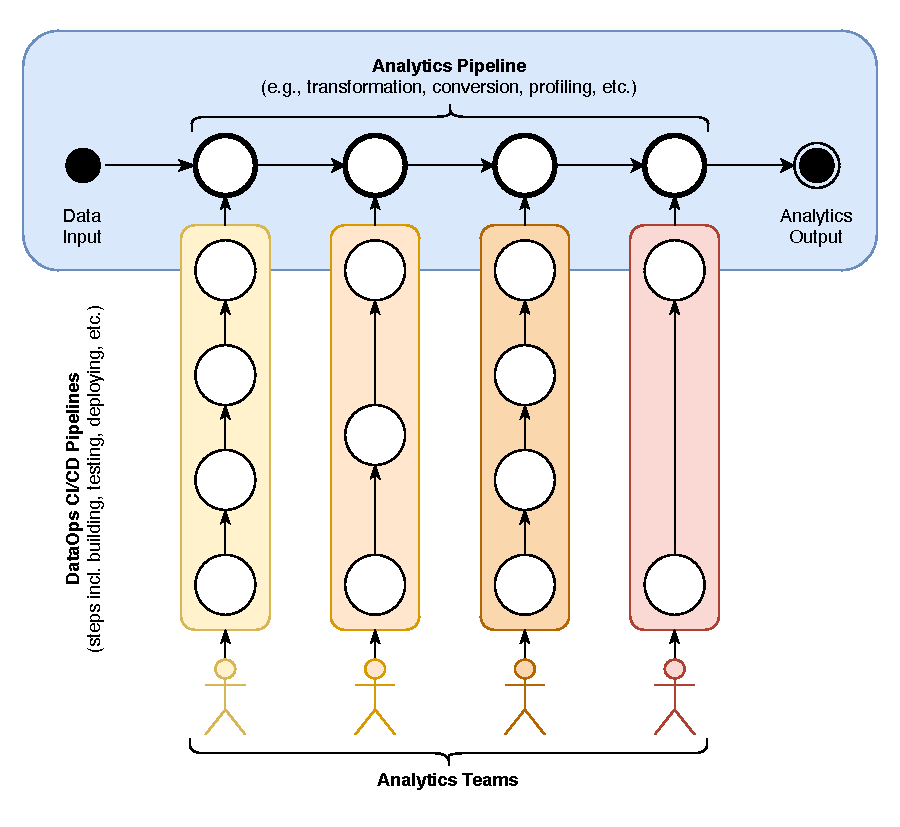
\includegraphics[width=\linewidth]{main-matter/img/2-1-2-pipeline-duality.pdf}
	\caption[DataOps Pipeline Duality]{DataOps Pipeline Duality (per \cite[38\psqq]{Bergh2019})}
	\label{fig:2-pipeline-duality}
\end{figure}

The data analytics (or data operations) pipeline is also called \textit{Value Pipeline} since it is in charge of answering questions through analytical insights \cite[32\psq]{Bergh2019}. Its horizontal representation visualizes its continuous flow. On the contrary, the vertical pipelines, also called \textit{Innovation Pipelines} represent the DataOps \ac{cicd} pipelines \cite[66]{Schmidt2019}. Whenever a new feature is developed for any stage of the pipeline, a number of preliminary steps is performed before finally deploying the solution into production \cite[33]{Bergh2019}. As with data analytics in general, the design of such pipelines highly depends on the analytics and quality requirements. In the scenario of Figure \ref{fig:2-pipeline-duality}, the individual stages require different \ac{cicd} steps and might also be worked on by different teams within the superordinate project.

As with DevOps, DataOps \ac{cicd} ties in with the project's \acf{vcs}. This allows for collaboration between developers as well as development environment management \cite{Davis2020}. Usually, a developer uses an individual sandbox to make changes to the common source code. This sandbox is a highly isolated environment which can be used without impacting the development process of other developers. It includes the current common source code as well as processes for installing and running all required dependencies \cite[41]{Bergh2019}. When committing a change to the \ac{vcs}, it triggers the corresponding \ac{cicd} pipeline which performs its checks and reports potential issues. Otherwise, the updated source code becomes the new common source code since the deployment into production has been conducted successfully.

Another methodology originating from DevOps is \textit{\ac{iac}}. In a desired automated environment, \ac{iac} also enables automatic creation, provisioning, and re-instantiation of a (cloud) infrastructure \cite[8\psqq]{Chaganti2018} which does not require repeated \ac{ui}-based configuration, etc. This is enabled by programatic configuration of infrastructure resources, settings, as well as applications.

\subsection{Agile Heritage: Fast-Paced, Iterative Development}
One problem within data analytics is that traditionally developed solutions cannot keep up with the demand of changing requirements. The development process is slow such that valuable and time-dependent information cannot be processed on time \cite{Lockner2019}. In software development, agile development mostly replaced traditional waterfall-orientated processes. \textit{Agile} in DataOps context means that development and improvement is iterative and fast-paced. It requires a \ac{mvp} which is continuously improved by means of previously mentioned \ac{spc} and \ac{cicd} processes \cite[19\psq]{Bergh2019}.

	\label{sec:2-dataops}
	
\section{Introduction to Testing}
	In general, software development relies on testing principles to holistically and objectively validate the expected performance of a piece of software. Neglecting testing in the discipline of software engineering might lead to customers and stakeholders of the solution loosing trust in its integrity and the increased occurrence of bugs and issues. In data analytics, the urge for testing is even stronger since errors in analytics outcomes might not only slow down business processes but have an enormous negative impact on data-reliant business decisions. An analytics solution might not crash and seemingly perform as expected but its resulting reports could contain errors that cannot be identified easily. DataOps-driven solutions also fall under this category, which is why these need to be ultimately tested for both software performance and data integrity.

To provide fundamental information on the testing principles required for designing a DataOps use case solution, the following sections define the integrity requirements of data analytics solutions (Section \ref{sec:2-1-requirements}), describe applicable frameworks and processes of both software and data testing, and eventually combine these by means of the DataOps methodology.



\subsection{Integrity Requirements of Data Analytics Solutions} \label{sec:2-1-requirements}
In order to define integrity requirements, the following section focusses on why results of data analytics processes are important, why bad data might impact these results, and what measures need to be taken into account for the solution to provide valuable analysis results.

Nowadays, organizations depend on data analytics more than ever \cite{Munawar2011}. \ac{bi} and \ac{dwh} solutions are designed to utilize data for business-required decision making \cite{Souibgui2019}. While these systems are expected to generate value, many companies lose trust in their data analytics because it might be prone to unforeseeable errors \cite{BISurvey.com}. This is because \ac{bi} and \ac{dwh} systems rely on high-quality data in order to provide representative analytics results and business insights \cite{Munawar2011}. Unfortunately, data quality issues of various sorts and manifestations lead to the systems generating false and potentially misleading reports \cite{Freudiger2014}\cite{Munawar2011}\cite{Redman2016}. Trying to reverse-engineer the preliminary data problems based on faulty analytics outcomes is not a valid approach. Instead, data quality is already required at its source to allow for efficient analytics and decision-making \cite{Redman2020}\cite{Tricentis}. Data quality assessment becomes increasingly harder due to an exponential rise in overall data volume in the past \cite{Freudiger2014}. Plus, complex analytics solutions are more fault-prone, which makes it harder to assess and find potential issues in their performance \cite{Homayouni2018}.

Addressing data quality issues needs to be a priority when performing analytics \cite{Freudiger2014}\cite{Veber2018}\cite{Redman2020}. Expecting blanket existence of data quality and, thus, not addressing it inside of the data analytics solution lifecycle, is a primary mistake \cite{Munawar2011}. Instead, data quality needs to be continuously assessed in each stage of such a solution. This includes the validation of the input data, testing for potential errors during data transformation, and making sure the output data complies with its origin \cite{Homayouni2018}\cite{Munawar2011}\cite{Redman2016}. Moreover, when multi-stage data analytics processes are utilized, the potential sources of errors is also multiplied, which requires individual testing of input, transformation, and output of each stage of the solution \cite{Homayouni2018}.

Data quality assessment needs not only to be performed for recently generated or required data, but for the entire database in use \cite{Redman2020}\cite{Freudiger2014}. Historic data is generally more prone to inconsistencies than recently acquired data since the former often originate from legacy systems, where infrastructure migrations might have lead to further quality issues \cite{Sneed2013}. This is especially crucial with \acs{ml}-driven applications since historical data is used for model training. If a model does not represent a specific situation correctly, its application for recent analyses will be inconclusive as well \cite{Redman2018}. Continuous monitoring of data quality issues within the utilization of \ac{bi} solutions could prove helpful for incremental improvement of outcomes \cite{Munawar2011}. Automation of the mentioned testing and validation processes increases productivity even more by reducing human error, accelerating detection, and introducing recovery measures within the conducted analyses \cite{Homayouni2018}\cite{Veber2018}.

All in all, data analytics solutions require tests regarding data quality at every stage where data is introduced, transformed, or processes. Furthermore, the software needs to report recognized issues and fall back into recovery protocols, if applicable. The automation of these measures is desired for better efficiency. Since data analytics solutions remain software product, the plain functionality needs to be assessed as well by means of traditional software testing and enriched with respect to data quality. 

\subsection{Software Testing}
Software testing is the process of analyzing the behavior of software, primarily to detect anomalies and defects that could be categorized as a software \textit{bug}. Software testing is conducted under controlled conditions and includes both positive and negative presets and a defined expected outcome for each testing use case \cite{Mahfuz2016}.

Software testing consists of various methods, types, and levels. The following section covers the relevant aspects of software testing for designing a testing concept within a data analytics solution.

\subsubsection{Testing Methods: Black Box vs. White Box Testing}
Testing methods are applied to decide the degree of abstraction of a test case. In general, either the \textit{Black Box} or the \textit{White Box} testing method is chosen. Black box testing is applied on test cases with a high degree of abstraction. The conducted test verifies the basic functionality of the application without considering its specific internal code logic. Therefore, creating such a test does not require deep knowledge of the specific code structure. The test literally treats the test candidate as a black box and checks if, given a specific input, a specific expected output is achieved \cite[65]{Mahfuz2016}

On the other hand, white box testing takes the internal code logic and structure into account. Its goal is to cover all possibilities of outcome, meaning to reach as many statements, condition checks and paths of the test candidate as possible. This implies that the test can only be written with good knowledge of the test candidate's source code operation. By conducting white box testing, not only expected behaviors are assessed by means of their final results. Instead, this testing method aims to confirm the internal integrity of the test candidate \cite[65]{Mahfuz2016}.

In general, both white-box and black-box testing can be leveraged for any level of software testing. In practice, black-box testing is more often used on higher levels of testing, as the internal integrity is expected to be tested on the lower levels, where white-box testing is rather utilized \cite[26]{Ammann2017}.

Introducing agility to testing is often seen as a testing method on its own \cite[70]{Mahfuz2016}. Since DataOps is conducted in an overall agile manner, non-agile methodologies of testing are not taken into consideration within this work.

\subsubsection{Testing Levels} \label{sec:2-2-2-levels}
Levels within software testing define the magnitude in which a test case is conducted \cite{Osherove2013}. These levels range from testing individual, granular software components in a highly controlled and isolated environment to global test runs of the overall behavior of the solution in its actual deployment environment \cite{Mahfuz2016}

\paragraph{Unit Testing} Unit testing is defined as the lowest level of software testing \cite[65]{Mahfuz2016}. As the name implies, the corresponding tests take individual components (i.e., \textit{units}) from the source code and check their behavior. Unit tests are pieces of code that invoke the chosen test unit and compare its actual result with the expected outcome \cite[sec. 1]{Osherove2013}. Depending on the test purpose, unit tests apply black box testing for basic functionality checks and white box testing for deeper internal functionality assessment. This requires detailed knowledge of the code under test \cite{Mahfuz2016}. Because of their granularity, a large number of unit tests is often required to test the software sufficiently. Thus, unit tests need to be of low complexity. They also need to be automated and repeatable, which requires a highly isolated test run environment. In general, unit test runs must perform idempotently. Each test needs to be able to run independently and cannot rely on outcomes of previous unit test runs. The unit test should reflect the intended usage of the test candidate, which also means that it needs to be relevant for the future of the code under test \cite[sec. 2]{Osherove2013}.

\paragraph{Integration Testing} Integration testing builds up on unit testing \cite[66]{Mahfuz2016}. Performing integration tests verifies that multiple combined units are working together as expected. It focusses on the testing of interfaces that connect singular components \cite[66]{Mahfuz2016} and is seen as an important counterpart to unit testing \cite[sec. 3]{Osherove2013}, since it covers areas that are usually not taken into account when performing isolated unit tests. Due to more dependencies outside of a controlled testing environment, the results of such tests might not be always consistent \cite[sec. 3]{Osherove2013} which implies the need for more abstract testing. It is also important that integration test only provide meaningful insights on the operation of the tested software when unit tests have been conducted and passed successfully. This is also emphasized in so-called \textit{incremental integration testing}. This process reflects the software development lifecycle by taking the addition of new features and components into account. The principle requires that the new or updated components are independently able to perform correctly before checking their integration in a higher-level testing combination \cite[66]{Mahfuz2016}.

\paragraph{End-to-End Testing} End-to-end testing is the highest level of software testing \cite[67]{Mahfuz2016} Usually, \textit{System Testing} is described as a level between integration and end-to-end testing. Since the underlying project is presented as a fundamental proof of concept for DataOps and contains a fairly simple system architecture, system tests do not lie inside the scope of this work. Aspects of system testing are also embodied inside end-to-end testing since it aims to be performed under (close-to) deployment requirements. This creates an idealized real-life scenario which makes use of external environments. Thus, end-to-end testing is the least isolated level and serves as the final test stage before actual deployment. Usually, this includes a run-through from start to finish \cite[67]{Mahfuz2016}. Again, end-to-end testing can only provide insightful measures about the integrity of a system when the lower test levels have passed successfully.

\subsubsection{Testing Types}
There are several testing types in software testing to further categorize the purpose of tests. Testing types either classify a subset of testing processes or are applied on top of them to increase its meaningfulness.

\paragraph{Functional Testing}
Functional testing verifies that software is created in compliance with its pre-defined, functional requirements \cite[69]{Mahfuz2016}. All traditional testing levels fall under the category of functional testing since they assess the general functionality of software and do not consider specific measures of how this functionality is achieved.

\paragraph{Non-Functional Testing}
Non-functional testing is the counterpart of functional testing \cite[69]{Mahfuz2016}. It verifies that the software achieves measures defined as non-functional requirements. This includes but is not limited to load, stress, or performance testing. While these terms are often used to describe similar activities \cite[70]{Mahfuz2016}, they have slightly different meanings. Load testing describes assessing the software's limitations based on heavy loads. Stress testing goes above these limits and does also take other factors of \textit{stress} into account (e.g., repetition of similar or identical processes, etc.). Performance tests are used for the long-term analysis of performance decrease over time \cite[70]{Mahfuz2016}. Other non-functional testing types include security and user experience. Since these aspects are not covered in this work, they are not further discussed here.

\paragraph{Regression Testing}
Regression testing is one of the most common testing types \cite[70]{Mahfuz2016} and can be found on each level of software testing \cite{Mathur2013}. It aims to uncover errors with pre-existing components when other components were newly included, changed, or removed. In other words, each part of the software must still perform correctly when a part of the features changed \cite[70]{Mahfuz2016}\cite{Mathur2013}. These tests are especially required when new releases are about to be deployed into production. Generally, regression tests are conducted for both corrective and progressive reasons, meaning that they can uncover current and potential future regression issues. To achieve regression testing in practice, unit tests can be written in a more abstract manner and re-run for the entire software solution, requiring older unit tests still to pass \cite{Mathur2013}. Thus, regression tests also highly benefit from automation \cite{Mahfuz2016}.

\paragraph{Smoke Testing}
Smoke testing describes a subset of test cases on several testing levels that assesses crucial, basic functionality of software. Smoke tests not passing can be an indicator for the core features of a (piece of) software not performing properly. They also imply that deploying the failing state of the software will most likely result in unrecoverable crashes. Using smoke tests allows for quick recognition of fundamental errors before performing other, much more granular tests \cite[sec. 5]{Tarlinder2016}.

\subsection{Data Quality Testing} \label{sec:2-2-3-data-testing}
The reasoning behind data quality testing is explained in the same manner as software testing: It ensures that the result of an analysis will be conducted properly and as expected as well as that problems are caught before they can cause any harm. In general, testing the data dimension of a data analytics solution ensures data quality \cite[2]{Savanur2016}. Other than with software testing, data quality testing does not rely on pre-defined and well-documented methods. Instead, the quality of the data in question needs to be purposefully defined based on its area of application \cite[1]{Askham2013}\cite{Schieferdecker2012}\cite[116\psq]{Sneed2013}\cite[667]{Souibgui2019}. This type of data governance provides rules \cite{Schieferdecker2012}\cite[116\psq]{Sneed2013} which can then be embedded inside the data analytics solution. 

\subsubsection{Dimensions of Data Quality}
Nevertheless, there are certain dimensions of data quality that are applied on the process of defining such rules. The \ac{dama} in the United Kingdom defined \enquote{The Six Primary Dimensions for Data Quality Assessment} in 2013 \cite[7\psqq]{Askham2013}. This section introduces these dimensions which will be used for defining data quality measures for the practical use case at hand at a later point of this thesis.

\paragraph{Completeness}
Data completeness describes the proportion of the stored data against the potential of being one-hundred percent complete \cite[8]{Askham2013}\cite{Shen2019}. It requires that there exists a definition for the \textit{whole} completeness of the data inside the given use case \cite[8]{Askham2013}. This is because an application might require certain data items and treat others as optional. An example for the lack of data completeness might be a personal data assessment form where the last name of a person is missing, even though the corresponding input field was marked required to be filled.

\paragraph{Uniqueness}
While completeness asks for (nearly) full data existence coverage, the data \textit{uniqueness} dimension requires it not to be more than that. Uniqueness is achieved when each unique data record only exists once inside the entire database at hand \cite[9]{Askham2013}. Several sources point out that duplicate data is a primary reason for misleading analyses, which means that achieving data uniqueness should be a top priority \cite{Shen2019}\cite[677\psq]{Souibgui2019}. An example for the lack of data uniqueness could be an employee database table listing 520 employees, even though only 500 people work at the given company.

\paragraph{Timeliness}
The timeliness of data is the degree to which data represents the reality from the required point in time. Whether a specific data record (or series of data records) is timely or not depends on the corresponding use case and data governance definition. This also includes the time difference of the creation of the data and its actual usage \cite[10]{Askham2013}. Depending on a use case, timeliness could be defined very strictly (e.g., for analyzing trends in stock trading markets) or rather loosely (e.g., changing the primary contact address of a person).

\paragraph{Validity}
Data validity describes a data item corresponding to its expected (and therefore, pre-defined) format, schema, syntax, etc. This definition should also include a range of expected or acceptable variation thresholds \cite[11]{Askham2013}. Testing for data schematics is one processes which allows for definitive objective differentiation between good and bad data \cite{Schieferdecker2012}. When a certain data item does not comply with its expected standards, it can be considered bad. Data validity provides metrics that can be included in the analytics process to efficiently rule out data quality issues without having thorough knowledge of the meaning of the data at hand \cite{Shen2019}.

\paragraph{Accuracy}
Data accuracy is the degree to which data \textit{correctly} describes the actual object or event existing in the real world. Defining data characteristics for accuracy can often be a long-term process which requires in-depth knowledge of the represented area of application \cite[9]{Askham2013}. Data accuracy goes hand-in-hand with data timeliness since outdated data can be a primary cause for bad data accuracy. Lack of accuracy might especially occur with invalid data entries that cannot be checked for \cite[12]{Askham2013}. One example might lay in the different date formats in the world. A user might presume the European data format (\texttt{DD-MM-YYYY}), even though the system requires U.S. date format (\texttt{MM-DD-YYYY}). As long as the input does not exceed the expected values, a syntactically correct but inaccurate data record is created.

\paragraph{Consistency}
Data consistency describes the absence of difference when comparing multiple representations of the same real-life object against its actual definition \cite[13]{Askham2013}. In other words, two occurrences of the same object do not differ if the object itself did not change between those occurrences. An example for data inconsistency might be two data records of identical purchases made by different customers where they are being charged different total amounts (discounts excluded).

\\\

These core dimensions can be enriched by taking other, more specific factors into consideration, e.g., data usability, data confidence, data value \cite[13\psq]{Askham2013}. It is also notable that the weighing of the respective dimensions strictly relies on the data analytics application \cite[5]{Askham2013}. This means that \textit{Timeliness} might be of great importance in one project, but could be neglected in another. Apart from that, certain dimensions \textit{cannot} be achieved without the existence of others, and other dimensions \textit{might} be achieved even if others are not.

\subsubsection{Data Quality Testing in Practice}
As mentioned inside the data quality dimension definitions, areas of data quality are mostly achieved when data complies with the corresponding data governance definitions. These allow for measuring the data quality \cite{Schieferdecker2012}. 

By including corresponding checks into the analytics software, not valuable data can be handled accordingly. These data quality checks are then performed before, during, and after the respective analysis. These checks must be designed in the same manner that can be seen in software testing: Either (a set of) data is good and passes the checks, or it it bad and fails \cite[1]{Savanur2016}, which then leads to analysis recovery measures, a program exit, etc. Additionally, data profiling \cite{GartnerGlossary3} could be used to fix recognizable and correctable issues. This could especially be useful with minor data quality inconsistencies, which might only cause problems when occurring in an extensive frequency. Plus, depending on the analytics context, some issues could even be neglected \cite[678\psq]{Souibgui2019}. Especially with data quality testing in multi-stage analytics pipeline environments, internal data lineage tracing is crucial in order to find out at which point the data failed its tests \cite{Shen2019}. Log files can then be used to reverse-engineer the data quality issue \cite{Askham2019}.

\\\

In conclusion, including  quality checks based on pre-defined data governance regulations, data quality issues could be recognized and handled accordingly. This could reduce the amount and severity of analytics reports resulting from bad data.

\subsection{Test Quality Measurement and Evaluation}
An important factor for testing, both for traditional software as well as data analytics solutions, is to measure the quality of the respective software and data tests \cite[30]{Brader2012}.

\subsubsection{Software Testing: Test Code Coverage}
A popular method for defining test quality in software development is to check how much code was executed during the run of a particular test suite \cite[30]{Brader2012}. It is expected that code with a high percentage of test code coverage will be less likely to contain unexpected faults. Microsoft suggests a code coverage of 80 percent or above for production-grade solutions \cite[30]{Brader2012}. On the other hand, high test coverage does not guarantee quality in code \cite[8]{Heckman2014}. This is because the execution of a code piece might have been invoked but the test suite did not perform any tests on this specific fragment. It is up to the developer to create tests that are not only aiming for a high coverage as the primary subject, but to consider all possible paths throughout the code under test \cite[9]{Heckman2014}.

There exist multiple categories of coverage that can point out lack of testing in certain areas. Based on the testing level, they can give insights on a specific code file, a specific area inside the code base or the entire code base in question.

\begin{description}
	\item[Line Coverage] defines the percentage of lines that have been called and executed without failure during the run of a test suite.
	\item[Statement Coverage] defines the percentage of statements that have been called and executed without failure during the run of a test suite \cite[2]{Heckman2014}. Other than with line coverage, a multi-line statement (e.g., definition and initialization of a large array, formatted for better readability) is considered singularly, which could improve the precision of the coverage.
	\item[Branch Coverage] checks if all paths of the code under test have been executed. This is important for conditions (i.e., \texttt{if/else if/else} statements) that need to be called in different scenarios to ensure coverage on the majority of execution cases \cite[2]{Heckman2014}.
	\item[Function/Method Coverage] represents the percentage of functions or methods that have been called and executed without failure during the run of a test suite \cite[2]{Heckman2014}. This process does not consider the importance or length of the functions or methods but can be used as an indicator if certain areas of the code have been left out of the testing suite entirely.
\end{description}
	
\subsection{Data Testing: Requirements Compliance}
As the findings of data testing in general (cf. Section \ref{sec:2-2-3-data-testing}) suggest, measurement of data testing quality strongly depends on the data governance requirements. All in all, it can be suggested that test cases should be designed to enforce tests inside crucial parts of the data definition, while optional or less application-areas could be treated less strictly. As with software test code coverage, a large number of data checks that inspect a large area of the data under test may not necessarily guarantee error-free data. It solely verifies that the tested areas will not make the analytics solution break or abort its processes. Moreover, the coverage is not expected to verify that analytics reports based on the allegedly clean data will be correct and insightful. The definition of high-quality data test cases is—again—up to the developer.
	

\subsection{Testing in DataOps}
As described previously in Section \ref{?}\todo{Add DataOps pipelines section}, DataOps contains a two-dimensional pipeline methodology. The Value Pipeline is used for the actual, real-time, production-grade analytics while the Innovation Pipeline continuously allows for feature updates of the analytics solution. The goal of DataOps testing is now to ensure correct and expected functionality of both dimensions \cite[40\psqq]{Bergh2019}. It is now to take the findings from the previous sections and to deduct an abstract, high-level framework for DataOps testing.

In general, the \enquote{Duality of testing in DataOps} \cite[40]{Bergh2019} now also requires two dimensions of tests which considers one of the two pipelines fixed, respectively. When testing the Value Pipeline, the underlying source code of the solution is fixed while various sorts of data are expected to flow through the pipeline. On the other hand, testing the Innovation Pipeline means checking for potential errors inside the analytics solution's update beyond its data. Here, the data is fixed (thus, pre-defined) and used to check whether the updated source code is ready to be deployed into production \cite[40]{Bergh2019}. 

\subsubsection{Value Pipeline: Data Quality Testing}
Various data flows through the Value Pipeline continuously. Traditionally, its goal is to take presumably valuable input data, perform various forms of data transformation and analysis, and report its output to some kind of knowledge base. With the findings on data quality testing (cf. Section \ref{sec:2-2-3-data-testing}), input data should not be presumed \textit{valid}. Now, another important purpose of the Value Pipeline is to conduct applicable data tests and enable measures if incorrect data is recognized. This process needs to be applied at each point where data is ingested, integrated, transformed or derived \cite{Layton2019}\cite{DataKitchen2020}. During the pipeline's performance, the source code (i.e., its features and modus operandi) do not change which is why it is the data stream that needs to be continuously verified. Enabling logging could allow for insightful operations processes finding the cause of the data problem.

\subsubsection{Innovation Pipeline: Software Testing}
The process within the Innovation Pipeline means the development and preparation of new features that are expected to improve the behavior of the analytics solution. Here, the validity of the new update needs to be validated by means of traditional software testing. In this case, using production-grade input data might not ensure the proper performance of the new solution. 

This is why the input data is prepared, taking various cases of data quality (based on the use case definition) into account. This set of test data should include \textit{bad data} which checks if the rejection and recovery measures of the new solution are in place. On the other hand, \textit{good data} needs to be provided \cite[234\psq]{Held2012} which will pass all data-related checks inside the source code and move on to the actual transformation and analysis steps, which then create output data that can be used for the analysis performance evaluation. In general, it is recommended to prepare generally applicable data based on the defined data governance specification rather than picking random data (with, thus, random errors) \cite[115]{Sneed2013}.

Plus, regression testing is a very important factor inside the Innovation Pipeline \cite{Shen2019} since data sets generated prior to the analytics solution update still need to be processable by the new release. Therefore, in case the update is based on a data format change, historic test data should also be included in the test data set. This can be seen as a parallel to pure software regression testing where previously designed unit tests are kept to ensure that a feature update does not collide with unchanged features. However, in case of a drastic feature change, the abstraction or complete removal of tests might be reasonable, depending on the architecture and specific feature update at hand.

\\\

In conclusion, holistic testing inside a DataOps environment is achieved by taking the change of both source code and data into account. The source code should contain a number of data quality checks based on its data governance specification. This approach of data quality testing is expected to allow for confidence in the analytics solution. On the other hand, the source code needs to be tested by means of traditional software testing methods, including the validation of the data quality checks and of all transformation and analysis actions. This is to be supported by an extensive test data repository which needs to be designed based on the production-grade data specifications. These tests are expected to invoke the majority of outcome possibilities, leading to a high test coverage and correct performance validation \cite{DataKitchen2020a}.

This testing duality concept is used for the design of the specific use case testing framework for this thesis' project in Chapter \ref{chap:dataops-testing}.


	\label{sec:2-testing}
	
\section{Technical Fundamentals}
	\subsection{Microservices}

\subsection{Python Programming Language}

\subsection{\acf{spc}}

\subsection{\acf{vcs}}

\subsection{\acf{cicd}}
	\label{sec:2-tech-fundamentals}
		\label{chap:theoretical-backgrounds}

	\chapter{Testing Framework Design Process}
		\input{main-matter/chapters/3-testing-framework/3-testing-framework.tex}
		\label{chap:testing-framework}

	\chapter{Analytics Pipeline DataOps Enablement}
		%===========================================================================
%	III. Analytics Pipeline DataOps Enablement
%===========================================================================

\section{Actual State Analysis: \acs{mba} Data Analytics Pipeline}
	\input{main-matter/chapters/4-dataops-enablement/4-1-analysis.tex}
	\label{sec:4-analysis}
	
\section{DataOps Enablement Requirements}
	\input{main-matter/chapters/4-dataops-enablement/4-2-requirements.tex}
	\label{sec:4-requirements}
	
\section{Architecture Design}
	\input{main-matter/chapters/4-dataops-enablement/4-3-architecture.tex}
	\label{sec:4-architecture}
	
\section{Modus Operandi}
	\input{main-matter/chapters/4-dataops-enablement/4-4-modus-operandi.tex}
	\label{sec:4-modus-operandi}
	
\section{Implementation}
	\input{main-matter/chapters/4-dataops-enablement/4-5-implementation.tex}
	\label{sec:4-implementation}
		\label{chap:dataops-enablement}

	\chapter{DataOps Testing}
		%===========================================================================
%	IV. DataOps Testing
%===========================================================================

\section{Testing Strategy}
	\input{main-matter/chapters/5-dataops-testing/5-1-strategy.tex}
	\label{sec:5-strategy}
	
\section{Testing Architecture Design}
	\input{main-matter/chapters/5-dataops-testing/5-2-architecture.tex}
	\label{sec:5-architecture}
	
\section{Implementation}
	\input{main-matter/chapters/5-dataops-testing/5-3-implementation.tex}
	\label{sec:5-implementation}
		\label{chap:dataops-testing}

	\chapter{Solution Evaluation}
		%===========================================================================
%	VI. Solution Evaluation
%===========================================================================

The following evaluation is expected to provide insights whether the solution works as intended during implementation. A focus is set on the testing capabilities of the \ac{cicd} pipeline in order to find potential limitations of the solution and discuss possible improvement techniques in theory. Throughout the evaluation, DataOps is compared to DevOps while focussing on the \ac{cicd} process and its testing features. This ultimately includes bottlenecks that cannot be covered by automated measures of the pipeline but rather need to be handled via conventions and best practices.

\section{Workflow Demonstration}
First of all, it might be valuable to evaluate the basic functionality of the \ac{cicd} pipeline, including its testing and deployment capabilities when no errors occur. For this matter, the general development workflow is applied. Before the following changes, the latest production-grade image was tagged with the commit ID \texttt{3c75dd5} inside \ac{ecr}.

A developer makes an arbitrary change to the Conversion Stage source code of the solution that is expected not to break the solution. This change is made in a separate feature branch of the \ac{vcs}. The developer can verify this fact by running the preexisting, automated tests locally on the developer sandbox. Then, a pull request is filed with the goal to merge the feature branch with the \texttt{master} branch, resulting in the new source code version being deployed into production. The pull request needs to include the appropriate GitHub labels, marking that the pull request should be treated as a new feature inside the Conversion \ac{cicd} pipeline. The filing could look like the screenshot provided in Figure \ref{fig:6-pr}. A pull request description is well-desired but omitted here for the sake of simplicity.
\newpage
\begin{figure}[h!]
	\centering
	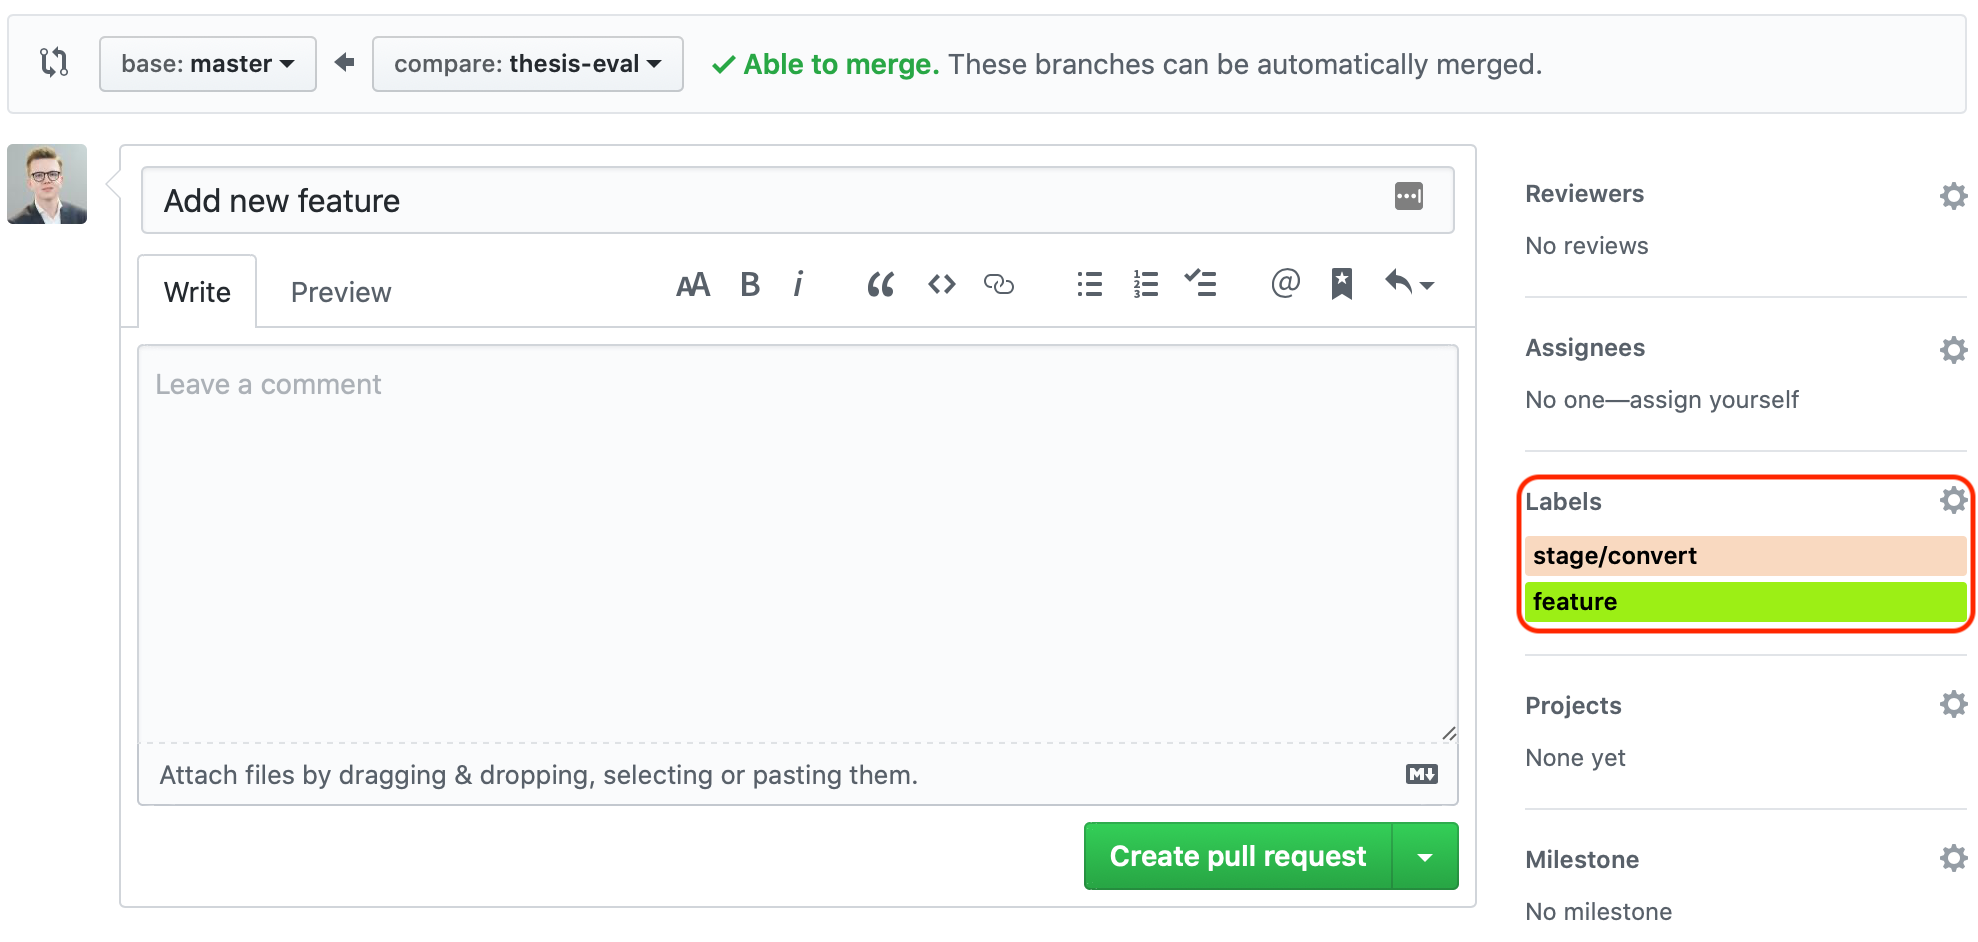
\includegraphics[width=\linewidth]{main-matter/img/6-pr.png}
	\caption{GitHub Feature Pull Request for Conversion Stage (Screenshot)}
	\label{fig:6-pr}	
\end{figure}

The first minor issue can be found inside this workflow. The developer in charge of this pull request is required to set the appropriate labels. The \texttt{feature} label missing would cause the \ac{cicd} pipeline not to run. The same applies to the stage specification label. An incorrect label could cause even more problems since this would trigger another pipeline with this stage source code, resulting in the build phase failing. The problem could be resolved by splitting up the repositories by stage but would remove the overall availability of the entire project's source code. This could have a negative impact on the productivity of the teams working on the project.

In case of correctly chosen labels, the Conversion Stage pipeline is triggered. A new pull request is automatically added to Jenkins and can be seen in the corresponding overview of the Jenkins \acs{ui}, shown in the screenshot in Figure \ref{fig:6-jenkins-pr}.

\begin{figure}[h!]
	\centering
	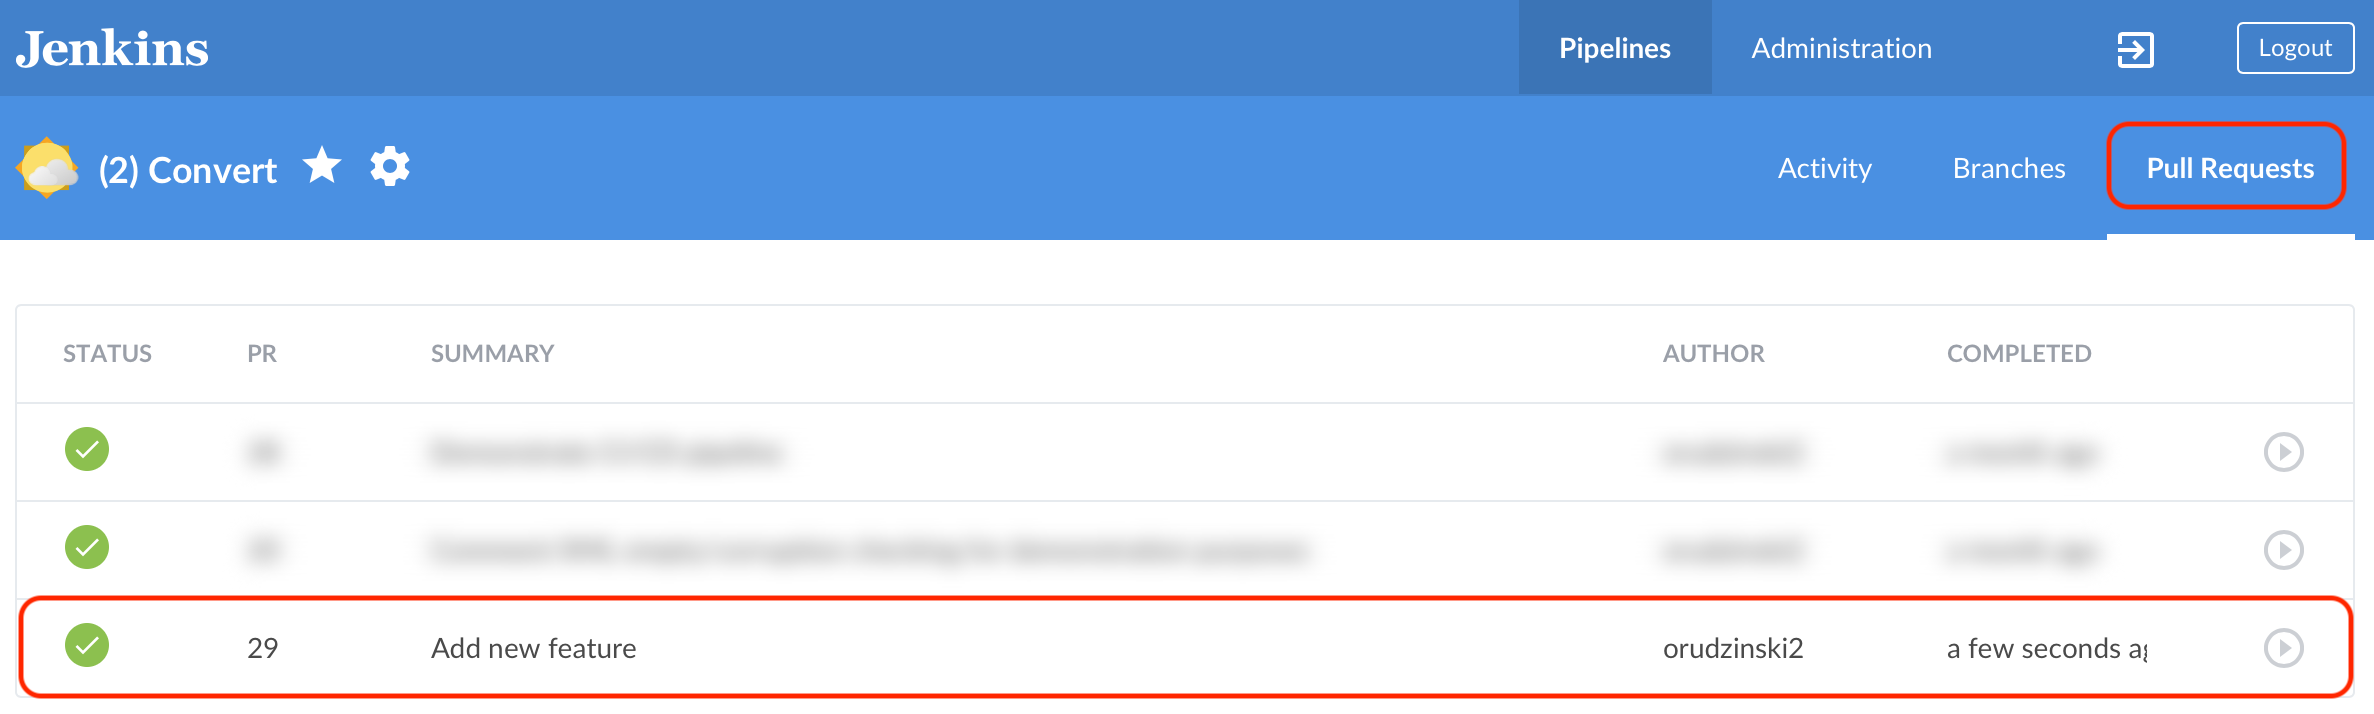
\includegraphics[width=\linewidth]{main-matter/img/6-jenkins-pr}
	\caption{Pull Request in Jenkins \acs{ui} (Screenshot)}
	\label{fig:6-jenkins-pr}
\end{figure}

The green checkmark shows that the pull request was evaluated, successfully verified and deployed. The specific pipeline overview can be retrieved by inspecting the corresponding pull request. This yields the following screenshot in Figure \ref{fig:6-jenkins-job-success}.

\begin{figure}[h!]
	\centering
	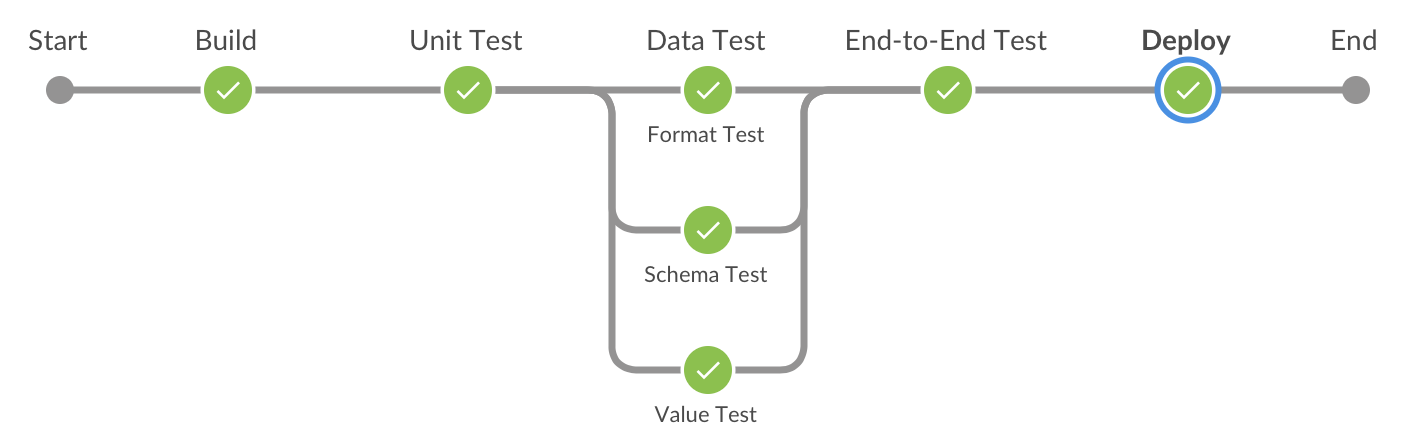
\includegraphics[width=\linewidth]{main-matter/img/6-jenkins-job-success}
	\caption{Successful Pipeline Job in Jenkins \acs{ui} (Screenshot)}
	\label{fig:6-jenkins-job-success}
\end{figure}

Since the deployment has run through correctly, \ac{ecr} should have received a new image. This image should be tagged with the last commit ID of the pull request as well as the \texttt{latest} tag. Inspecting the corresponding repository inside the \ac{aws} Console verifies this claim, presented in the screenshot of Figure \ref{fig:6-ecr}

\begin{figure}[h!]
	\centering
	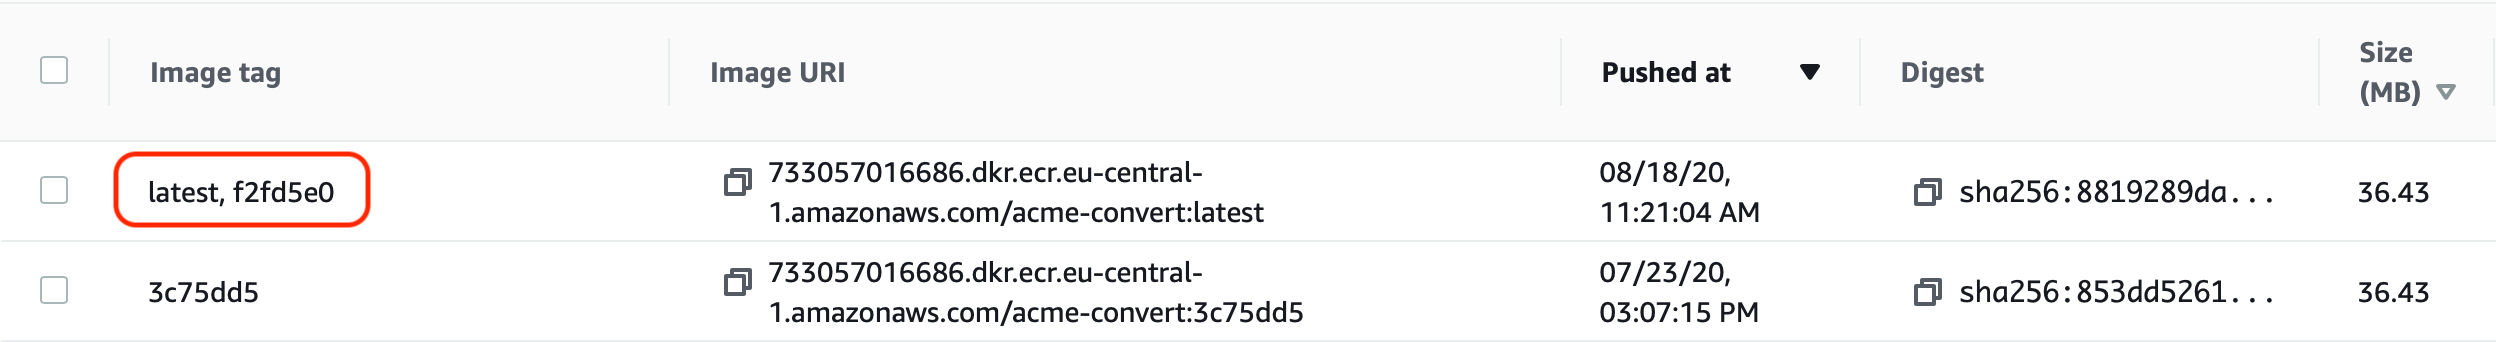
\includegraphics[width=\linewidth]{main-matter/img/6-ecr}
	\caption{Image List of the Conversion Stage \acs{aws} \acs{ecr} Repository (Screenshot)}
	\label{fig:6-ecr}
\end{figure}

It can be seen, that the new image has been included with the appropriate tags. The old version of the image still resides in the repository for versioning reasons. Because of the correct tagging, Airflow will use this updated version of the Conversion Stage image for upcoming analyses. 

The source code change is not reflected in the GitHub repository, yet. The feature branch still exists and the \texttt{master} branch has not been changed. Since the required \ac{cicd} checks have run through successfully, the developer can now merge the feature branch with the \texttt{master} branch. This manual procedure is required by GitHub. This can be seen as another issue of lacking automation since the developer may not forget to merge the branches and remove the feature branch after the deployment has been conducted successfully. Existing copies of the previous \texttt{master} branch inside other development sandboxes need to be updated now since working with the outdated version might cause compatibility issues of upcoming versions as well as so-called \textit{merge conflicts} within GitHub, where the feature might be correct by means of the \ac{cicd} evaluation, but the code history of the branches to merge does not allow for an automatic merge and requires manual correcting.

At this point, one iteration of the \ac{cicd} workflow is completed.

\section{Testing Capability Evaluation}
The previous evaluation use case does intentionally not contain issues in order to demonstrate the desired development workflow. Now, the workflow of the pipeline is evaluated for different kinds of issues. In general, this is divided into two categories:

\begin{enumerate}
	\item issues that result from updating existing features, and
	\item issues that result from creating new features.
\end{enumerate}

\subsection{Feature Update Testing}
The most na\"ive approach is to remove a line of code that is required by the testing framework. This simulation is comparable to a scenario where an existing feature is updated but a required functionality was removed. The testing framework is supposed to be invoked by the \ac{cicd} pipeline job and catch the issue. Specifically, the line checking for a corrupted \ac{xml} file inside the analytics script of the Conversion Stage is removed. This data handling function has been presented in Section \ref{sec:5-3-3-2}.

The process of filing a pull request remains identical. Jenkins' pull request job is triggered again, resulting in the job workflow depicted in the screenshot in Figure \ref{fig:6-jenkins-pr-fail1}.

\begin{figure}[h!]
	\centering
	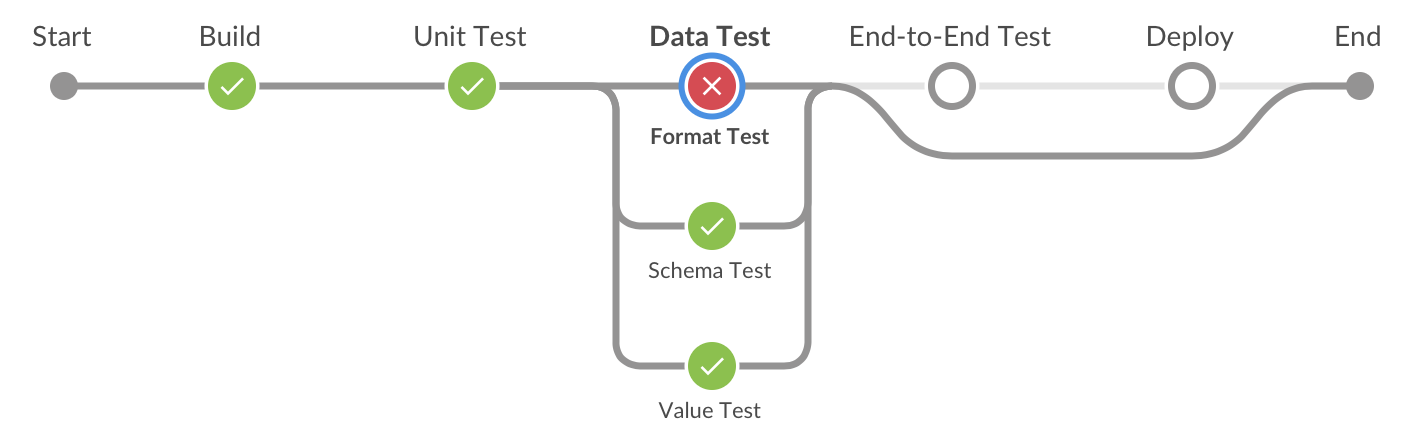
\includegraphics[width=\linewidth]{main-matter/img/6-jenkins-pr-fail1}
	\caption{Failing Pipeline Job in Jenkins \acs{ui} (Line Missing) (Screenshot)}
	\label{fig:6-jenkins-pr-fail1}
\end{figure}

Since \ac{xml} corruption testing is subject to the data format testing suite, the corresponding stage inside the \ac{cicd} pipeline fails. The upcoming stages are skipped such that no flawed deployment is conducted. The \textit{Tests} tab of the job inside the Jenkins \ac{ui} provides insights to the tests that have been run during the testing stages and highlights tests that did not pass. This overview is shown in a screenshot in Figure \ref{fig:6-jenkins-tests}.
\newpage
\begin{figure}[h!]
	\centering
	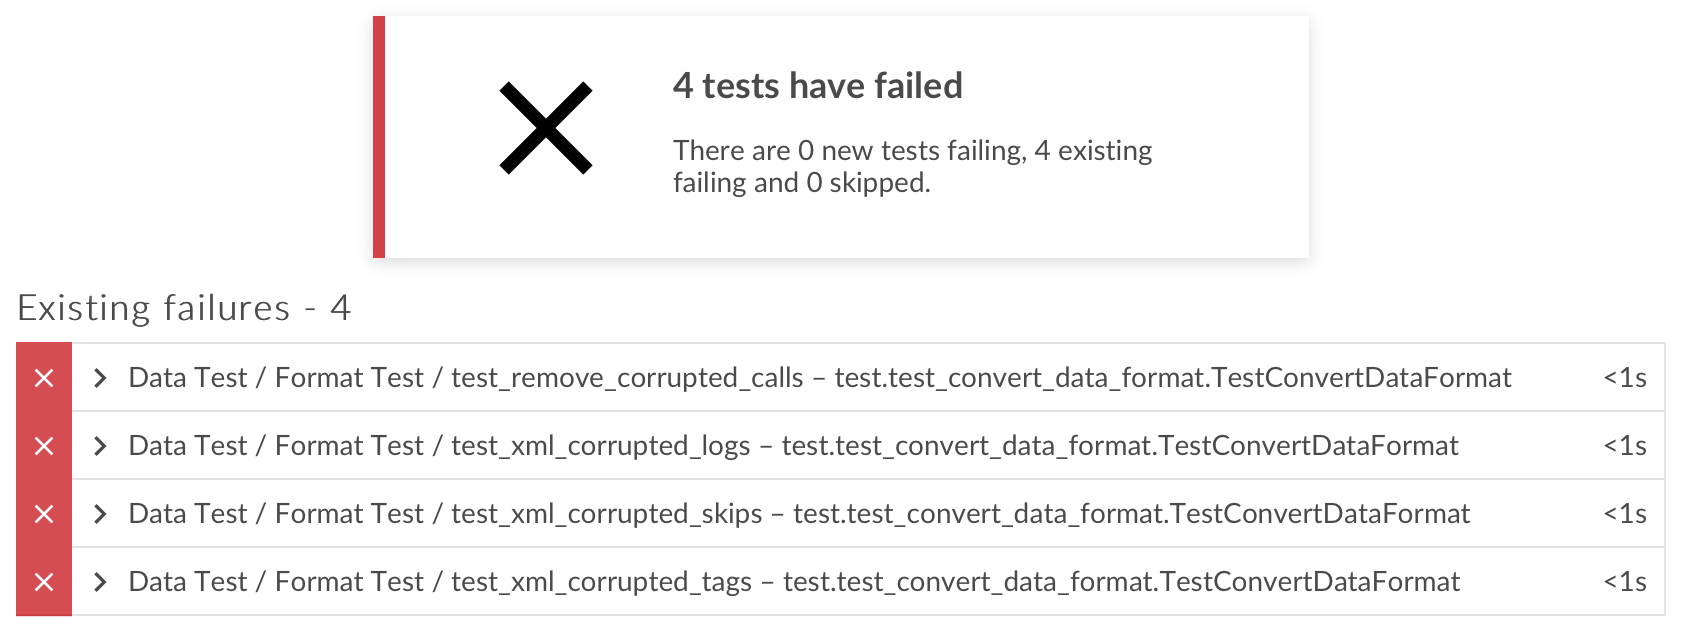
\includegraphics[width=\linewidth]{main-matter/img/6-jenkins-tests}
	\caption{Failing Tests in Jenkins \acs{ui} (Line Missing) (Screenshot)}
	\label{fig:6-jenkins-tests}
\end{figure}

It can be seen that all tests regarding \ac{xml} corruption fail. This is because the centralized \texttt{remove\_corrupted(...)} data handling function is not called inside the analytics script anymore. Since all handling measures are defined in that function, no measure is actually taken when the function call is missing. In case of the data handling function missing individual handling steps, the corresponding tests would fail. These test results are meant to provide valuable insights to the developer. The developer can analyze the problem, fix occurrences, and push a new commit to the pull request. When the test failures have been resolved, the updated version can be correctly deployed.

Similar failure detections occur with different changes of the source code. This shows that the pipeline is capable of stopping a deployment process based on the existing tests. This requires the assumption that all tests suites are complete and perform as expected.

\subsection{Feature Creation Testing}
The previous paragraphs cover the integration of an already existing feature. The following paragraphs deal with the creation and adequate testing of a new feature. The consideration of this practical area is important since the solution at hand can encounter changing requirements that need to be embodied accordingly.

For this evaluation, assume that the product owner of the \ac{mba} data pipeline requests a new feature that includes the weather data of the creation date of the purchase information to the analysis. This could be used to find a possible correlation between the purchasing behavior of the retail company's customers and the weather situation at the given point in time. The development teams find that the integration of weather data is mostly suited to be developed inside the Conversion Stage of the data pipeline since it represents the first stage that has access to the raw purchasing data.

The na\"ive implementation of that feature is shown in Source Code Excerpt \ref{src:6-weather} below.

\begin{listing}[h!]
	\inputminted{python}{main-matter/src/6-weather.py}
	\caption{Na\"ive Implementation of a Weather Data Integration Feature}
	\label{src:6-weather}
\end{listing}

The feature's corresponding function is placed right after the reformatting of the \ac{pos}Log dictionaries and, thus, right before the \ac{json} file export. For each purchase, the weather that corresponds to the transaction date and place is requested from an external weather \acs{api} (ll. 5--12). For simplicity reasons, the average weather data in degrees Celsius is extracted (ll. 14--16) and added to the dictionary (l. 18). There are multiple issues that can occur when such a code fragment is integrated to the solution. 

\subsubsection{Feature Testing Limitations}
When performing an update of an existing feature, the validation of the update can be conducted by running the preexisting tests of the corresponding feature. However, the development of a new feature also means writing new tests. The \ac{cicd} pipeline can only stop a feature from being deployed into production when corresponding feature tests fail. In case that these tests do not exist, the \ac{cicd} pipeline cannot recognize any issues and publishes an untested feature. This situation is highly undesired and problematic for the integrity of such a solution. Plus, it yields discussions that go beyond the technical aspects of data analytics development but need to deal with the developer's understanding and acceptance of an agile development workflow.

In agile development, a developer is always in charge of testing the feature that he or she works on \cite[18]{Kaiser}. Principles like \ac{tdd} have been introduced to support the importance of the testing process \cite[1]{Karac2018}. DataOps testing principles might develop this into a data-driven approach (i.e., test data first, then solution test, then feature implementation). Nevertheless, from a general point of view, these principles can be suggested or required by convention, but not technically enforced. A separate tool could evaluate if tests exist for a given feature by executing all test suites and calculating the feature's occurrences in these tests. This measurement is referred to as the \textit{test code coverage} \cite[15]{Garrett2011}. However, such a mechanism could be bypassed by simply executing a function inside a test case. This could presume the feature being tested and allow the change to be deployed into production. Other, more complex metrics (e.g., defect fix retest, test effectiveness, etc. \cite[15]{Garrett2011}) could be suited for more in-depth testing quality assurance, but would still be required to be implemented and reevaluated for the given use cases over time.  All in all, DataOps requires the acceptance and consciousness of agile processes and does not only rely on technical measurements to control their fulfillment.

Even with appropriate testing, the issue is still present. This is because the feature and the corresponding tests are conducted by human developers. The person behind a feature might have a different understanding of the feature than the product owner or simply miss an edge case during testing that could lead to further issues. Specifically, the developer might implement the feature to provide weather data in degrees Fahrenheit and test the value correctness accordingly. The product owner or other developers might expect degrees Celsius instead. As with pure software development, such a feature change also requires updating the solution requirements and general collaboration and communication between developers and development teams of the separate stages. In general, all contributors should have the same understanding of a feature in order to prevent inconsistencies.

This issue also introduces the discussion of \textit{testing tests} that are meant to test the functionality of the source code. The addition of testing validation based on previously mentioned complex testing quality metrics might mean more effort. With these validation systems, the question behind \textit{their} validity can be posed and the discussion continues. This ultimately means that automated tests might not suffice for confident and correct deployment of such a solution. Apart from that, peer code reviews and other interdisciplinary measures might need to be taken in order to rule out mistakes that cannot be uncovered by traditional software solution testing.

\subsubsection{Importance of Regression Testing}
Another issue can be found in regression. Assume that a previous \ac{mba} needs to be re-conducted because an error inside its values is suspected. The data from the target \ac{mba} originates from a time before this feature was requested. The previous \ac{mba} did also not consider weather data for its analysis. When the analysis is repeated, the \ac{mba} might, purposefully, yield different results. However, this behavior is not desired. The addition of a new feature shall not lead to inconsistencies between two versions of the same analysis. This would create a new data quality issue and result in further issues in the upcoming analytical stages. Instead, this feature may only be used for new analyses (e.g. by specifying a minimum date that needs to be present in the input data). This behavior correctness needs to be ensured by including a corresponding test to the testing suite of the solution.

Another form of regression testing in this case is the execution of previous tests. Their passing will ensure that the new feature does not change the behavior of previously existing features. Since this feature only adds an attribute to the output of the stage, the previous features and feature tests run correctly. Other feature implementations might require the change of preexisting features which then might require the adaptation of the corresponding tests, etc. \\\

All in all, the general testing process, including its limitations and technical bottlenecks, can be compared to agile DevOps testing. On the other hand, regression testing plays a priority role in data analytics testing and needs to be taken into account for each feature. This finding preliminarily corresponds with the hypothesis from Section \ref{sec:2-2-innovation-pipeline}. Currently, it can be said that the DataOps testing process is similar to DevOps, but takes data-specific requirements into account.

\section{Impact Analysis of Different Testing Levels}
In order to evaluate further potential differences to the DevOps testing process, the following section deals with the different testing levels (unit, integration, and end-to-end testing) in the \ac{mba} DataOps pipeline environment. This part of the evaluation is expected to yield insights about the specific impact of the testing levels in such a data-driven environment, built up in a highly externalized technical infrastructure. 

This evaluation is conducted based on testing use cases that occur at different hierarchical levels of the testing process. These use cases are not explicitly tested for by the solution. The evaluation will provide information on how insightful the error recognition of the different testing levels is for recovering from the problem. The use cases are described as follows:

\begin{description}
	\item[Non-Existing \ac{s3} Bucket \acs{uri} Provided] The format of the \ac{uri} is correct, but the bucket does not exist (typographic error, deprecated bucket reference, etc.).
	\item[Invalid \ac{aws} \ac{iam} Credentials Provided] The format of the \ac{iam} credential key pair is correct, but it either does not provide sufficient access to the resources, or it is deprecated .
	\item[Container Task Ran Out of Memory] The container that an analytics stage is run in cannot finish its job because it requires more memory than expected.
\end{description}

\subsection{Failure Case Execution}
These cases are designed and invoked, leading to the following results:

\subsubsection{Non-Existing \ac{s3} Bucket \acs{uri} Provided}
\begin{table}[h!]
\centering
\begin{tabular}{r!{\vrule width 1pt}l|l|l}
\multicolumn{4}{c}{\textbf{Non-Existing \acs{s3} Bucket \acs{uri} Provided}}                                                                        \\[0.4em] \ChangeRT{1pt}
\makecell[r]{\textbf{Level}}       & \textbf{Unit} & \textbf{Integration}                                                       & \textbf{End-to-End} \\ \ChangeRT{1pt}
\makecell[r]{\textbf{Result}}      & \cellcolor{green!25}passed        & \cellcolor{red!25}failed                                                                     & \cellcolor{gray!25}\textit{skipped}                \\ \hline
\makecell[r]{\textbf{Information}} &               & \makecell[l]{\texttt{boto3} Exception:\\ \texttt{404 Not Found}} &                    
\end{tabular}
\caption{Testing Evaluation: Non-Existing \acs{s3} Bucket \acs{uri} Provided}
\label{tab:6-bad-s3}
\end{table}

As can be seen in Table \ref{tab:6-bad-s3}, the corresponding unit test only tests if \ac{s3} \acsp{uri} of incorrect format are caught and reported. Since the \acs{uri} at hand is correct, the unit test passes. The integration (data) test actually connects to the bucket, resulting in an \texttt{boto3} exception, reporting that the provided \ac{s3} bucket does not exist.

The process of mocking the \ac{s3} connection service inside the unit test would not have helped here since the actual existence of the infrastructure can only be evaluated \textit{within} the scope of the infrastructure.
\newpage
\subsubsection{Invalid \ac{aws} \ac{iam} Credentials Provided}
\begin{table}[h!]
\centering
\begin{tabular}{r!{\vrule width 1pt}l|l|l}
\multicolumn{4}{c}{\textbf{Invalid \ac{aws} \ac{iam} Credentials Provided}}                                                                        \\[0.4em] \ChangeRT{1pt}
\makecell[r]{\textbf{Level}}       & \textbf{Unit} & \textbf{Integration}                                                       & \textbf{End-to-End} \\ \ChangeRT{1pt}
\makecell[r]{\textbf{Result}}      & \cellcolor{green!25}passed        & \cellcolor{red!25}failed                                                                     & \cellcolor{gray!25}\textit{skipped}                \\ \hline
\makecell[r]{\textbf{Information}} &               & \makecell[l]{\texttt{boto3} Exception:\\ \texttt{Access Denied}} &                    
\end{tabular}
\caption{Testing Evaluation: Invalid \acs{aws} \acs{iam} Credentials Provided}
\label{tab:6-bad-iam}
\end{table}
This case is similar to the incorrect \acs{uri} and results in the same test outcome, shown in Table \ref{tab:6-bad-iam}. Only the infrastructure itself can evaluate the credentials and report an issue. This is why, again, the unit test passes, while the integration test results in another exception, mentioning that the provided credentials cannot be used for the current operation.

\subsubsection{\acs{ecs} Container Task Ran Out of Memory}
\begin{table}[h!]
\centering
\begin{tabular}{r!{\vrule width 1pt}l|l|l}
\multicolumn{4}{c}{\textbf{\acs{ecs} Container Task Ran Out of Memory}}                                                                        \\[0.4em] \ChangeRT{1pt}
\makecell[r]{\textbf{Level}}       & \textbf{Unit} & \textbf{Integration}                                                       & \textbf{End-to-End} \\ \ChangeRT{1pt}
\makecell[r]{\textbf{Result}}      & \cellcolor{green!25}passed        & \cellcolor{green!25}passed                                                                     & \cellcolor{red!25}failed                \\ \hline
\makecell[r]{\textbf{Information}} &               &  & \makecell[l]{\texttt{boto3} Exception:\\ \texttt{OutOfMemoryError: Container killed}\\\texttt{due to memory usage}}                  
\end{tabular}
\caption{Testing Evaluation: \acs{ecs} Container Task Ran Out of Memory}
\label{tab:6-oom}
\end{table}
In this case, both the unit and integration tests do not recognize the problem. Only the end-to-end test provides the information that the corresponding \ac{ecs} task has failed because of lacking memory capacity, shown in Table \ref{tab:6-oom} This is because the integration tests are performed in containerized environments on the Jenkins server instance. These Docker containers do not have any resource limitations \cite{docker}, in contrast to the \ac{ecs} tasks that require performance specifications in their definitions. Only the end-to-end test makes use of this infrastructural service inside the solution.
\newpage
\subsection{Testing Impact Evaluation}
The presented use cases yield a number of insights. First, the typical, DevOps-inspired testing level hierarchy and its degrees of testing isolation do not hold in an environment that is mostly created out of external resources. The cloud-driven infrastructure cannot be taken into account by unit tests since these are supposed to neglect these aspect and purely focus on the feature under test. When the infrastructure access is a crucial component of the feature, the unit test cannot recognize any issues.

Another aspect that follows is the strict separation of the testing levels. Taking the findings of the failure use cases into account, all infrastructure-related testing might be conducted during integration testing. This could also include \acs{uri} and \acs{iam} credential format tests that do not require infrastructure access but categorically fit inside the same testing suite. This aspect has partly been considered during development: certain data handling function tests could have been created in the domain of granular unit tests. Since their overall features relate to the data-driven part of the solution, which has been tested during integration testing, the remaining tests are performed similarly.

Finally, the last failure use case that was only recognized by end-to-end testing opens up another discussion topic. In general, the performance measures could have been implemented into the integration testing level that makes use of Jenkins-driven Docker containers. This would require additional testing effort and, potentially, the redesign of the deployment structure within the \ac{cicd} pipeline. While the overall reason behind testing should be the validation of feature functionality, strictly focussing on the definition of the testing levels could increase time and cost inside the development process.

As emphasized throughout this entire work, DataOps use cases and their corresponding automation and testing designs highly differ depending on the solution requirements, data governance definitions, etc. For the \ac{mba} data pipeline, unit tests provide little value to the actual testing expressiveness. There exists a general discussion questioning the value of unit tests \cite{Coplien}\cite{Golub2020}. This finding goes hand-in-hand with this discussion. On the other hand, unit testing allows for better testing performance. When the practice of \textit{mocking} external services (i.e., mimicking the required service functionality inside the local test case) is exhausted, this performance benefit vanishes due to increasing testing design complexity. The unit test cases might be included into the integration testing area and de-granularized for potentially better testing productivity. Further evaluation could give more insights on the impact differences between integration and end-to-end testing, leading to a generally more specialized, efficient and less tradition-driven testing architecture. 

All in all, it is proposed that DataOps tests are categorized semantically regarding their meaning for the solution rather than focussing on testing level syntax. Furthermore, testing design needs to be weighted up between the creation complexity of isolated tests as well as the urge for isolated unit test cases. \\\

In generalization and comparison to the DevOps testing process, it can still be said that automated testing is performed inside its designated steps inside the \ac{cicd} process prior to deployment. However, data analytics solutions often have to deal with externalized services, that cannot be neglected during testing. Instead of sticking to the traditional testing pyramid, each solutions' architecture needs to be evaluated from a testability point of view in order to create a well-suited testing framework inside the DataOps use case.




		\label{chap:solution-evaluation}
	
	\chapter{Conclusion}
		%===========================================================================
%	VII. Conclusion
%===========================================================================

This final chapter retrospects on the work and findings inside this bachelor's thesis. It started out with background information on DataOps and testing methodologies. It conducted an actual state analysis of a preexisting, static \ac{mba} data analytics solution based on the state-of-the-art findings. This determined action items for the DataOps enablement and testing enhancement of the solution. The thesis then proposed a general DataOps testing framework and applied its steps on the Conversion Stage of the data pipeline in theory. Then, the DataOps process and testing framework have been practically implemented. Finally, the new solution was evaluated by means of the key goals of this thesis, being the understanding of DataOps testing, similarities and differences to DevOps testing, as well as limitation of the solution.

\section*{Key Findings} \addtocounter{section}{1}
During research, design, implementation, and evaluation, the following key characteristics were found:

As with traditional software solution testing, data analytics testing supports the quality of new version releases. It provides confidence in the product for all stakeholders, leading to less post-deployment issues, and therefore, to less cost, time, and risk during production-grade usage. Eventually, well-tested data analytics solutions are expected to provide more valuable business insights for the organizations that take advantage of them.

Moreover, DataOps testing is an inherent part of DataOps that benefits from technical support through automation and the separation of execution environments. Nevertheless, DataOps remains an agile work model that requires an adequate agile mindset. The DataOps \ac{cicd} pipeline can only recognize test failures with actually available tests. If a developer team decides to neglect testing and work around potential testing mechanisms, there will be no tests that could fail, resulting in a passing deployment. From a qualitative point of view, this is unacceptable but could not be realistically enforced with additional technical measures. Instead, testing conventions and best practices should be known and accepted by the performing developers. Then, DataOps testing can be very valuable for correct and confident solution development and deployment.

Even with the required agile mindset, test quality might be an issue. Since these tests are written by human developers, they might not take certain edge cases into account, leading to an insufficiently tested solution. Again, test quality measurements could be implemented into the solution but should also be supported by non-automated processes, like peer code reviews, etc.

The testing design process should consider that historic analyses might need to be re-conducted, aiming for consistent results regardless of the current version of the data analytics solution. Therefore, regression testing and the conditional execution of features need to be taken into account.

While DataOps testing can be achieved by utilizing traditional software testing tools, it does not follow the exact same process of DevOps testing. Since data analytics solutions often depend on a variety of external services, these also need to be considered during testing. This goes against the traditional testing pyramid that aims for isolated, granular unit tests. Instead, DataOps tests should not strictly stick to the traditional testing levels but provide semantically categorized testing suites that reflect the desired workflow of the solution.

\section*{Proposal for Further Research} \addtocounter{section}{1}
The preliminary goal of the thesis' project was to demonstrate the discipline of DataOps testing by means of an exemplarily chosen data analytics scenario. Throughout the research and development process, it became clear that different types of data analytics projects are expected to have different types of requirements. It might be reasonable to evaluate the testing design framework and process inside other use cases, using different technologies. For instance, it is expected that more complex, \acs{ml}-driven data analytics will require additional infrastructure and testing methodologies. Furthermore, analytics derived through \acs{ml} might need additional testing attention regarding ethical questions. In general, the solution at hand covers deterministic testing. It might be of great interest to find out how such testing is conducted with predictive data analytics. \newpage

Picking up on the test quality issue finding from this thesis, implementation and evaluation of test quality assurance measures might concretize if testing conventions can be reasonably supported by automated mechanisms. \\\

In conclusion, the demonstration of \ac{mba} DataOps testing underlined the importance and capability of data analytics development and testing automation. With further research and development based on this work, generally applicable DataOps testing frameworks and tools for a variety of use cases and complexities could be created, resulting in better data analytics solutions and outcomes for organizations throughout several industries.
		\label{chap:conclusion}
		
		
%===========================================================================
%	BACK MATTER
%===========================================================================

	\pagestyle{plain}
	\clearpage
	\pagenumbering{alph}
	\printbibliography
\end{document}